% \hfill between subfigures — horizontal fill, pushes the next subfigure away, distributing leftover space evenly.


\documentclass{article}
\usepackage{graphicx}   % MANDATORY for \includegraphics to work
\usepackage{subcaption} % For subfigures

\begin{document}

\begin{figure}[htbp] % Changed [h] to [htbp] for better layout flexibility
  \centering
  \begin{subfigure}{0.3\textwidth}
    \centering
    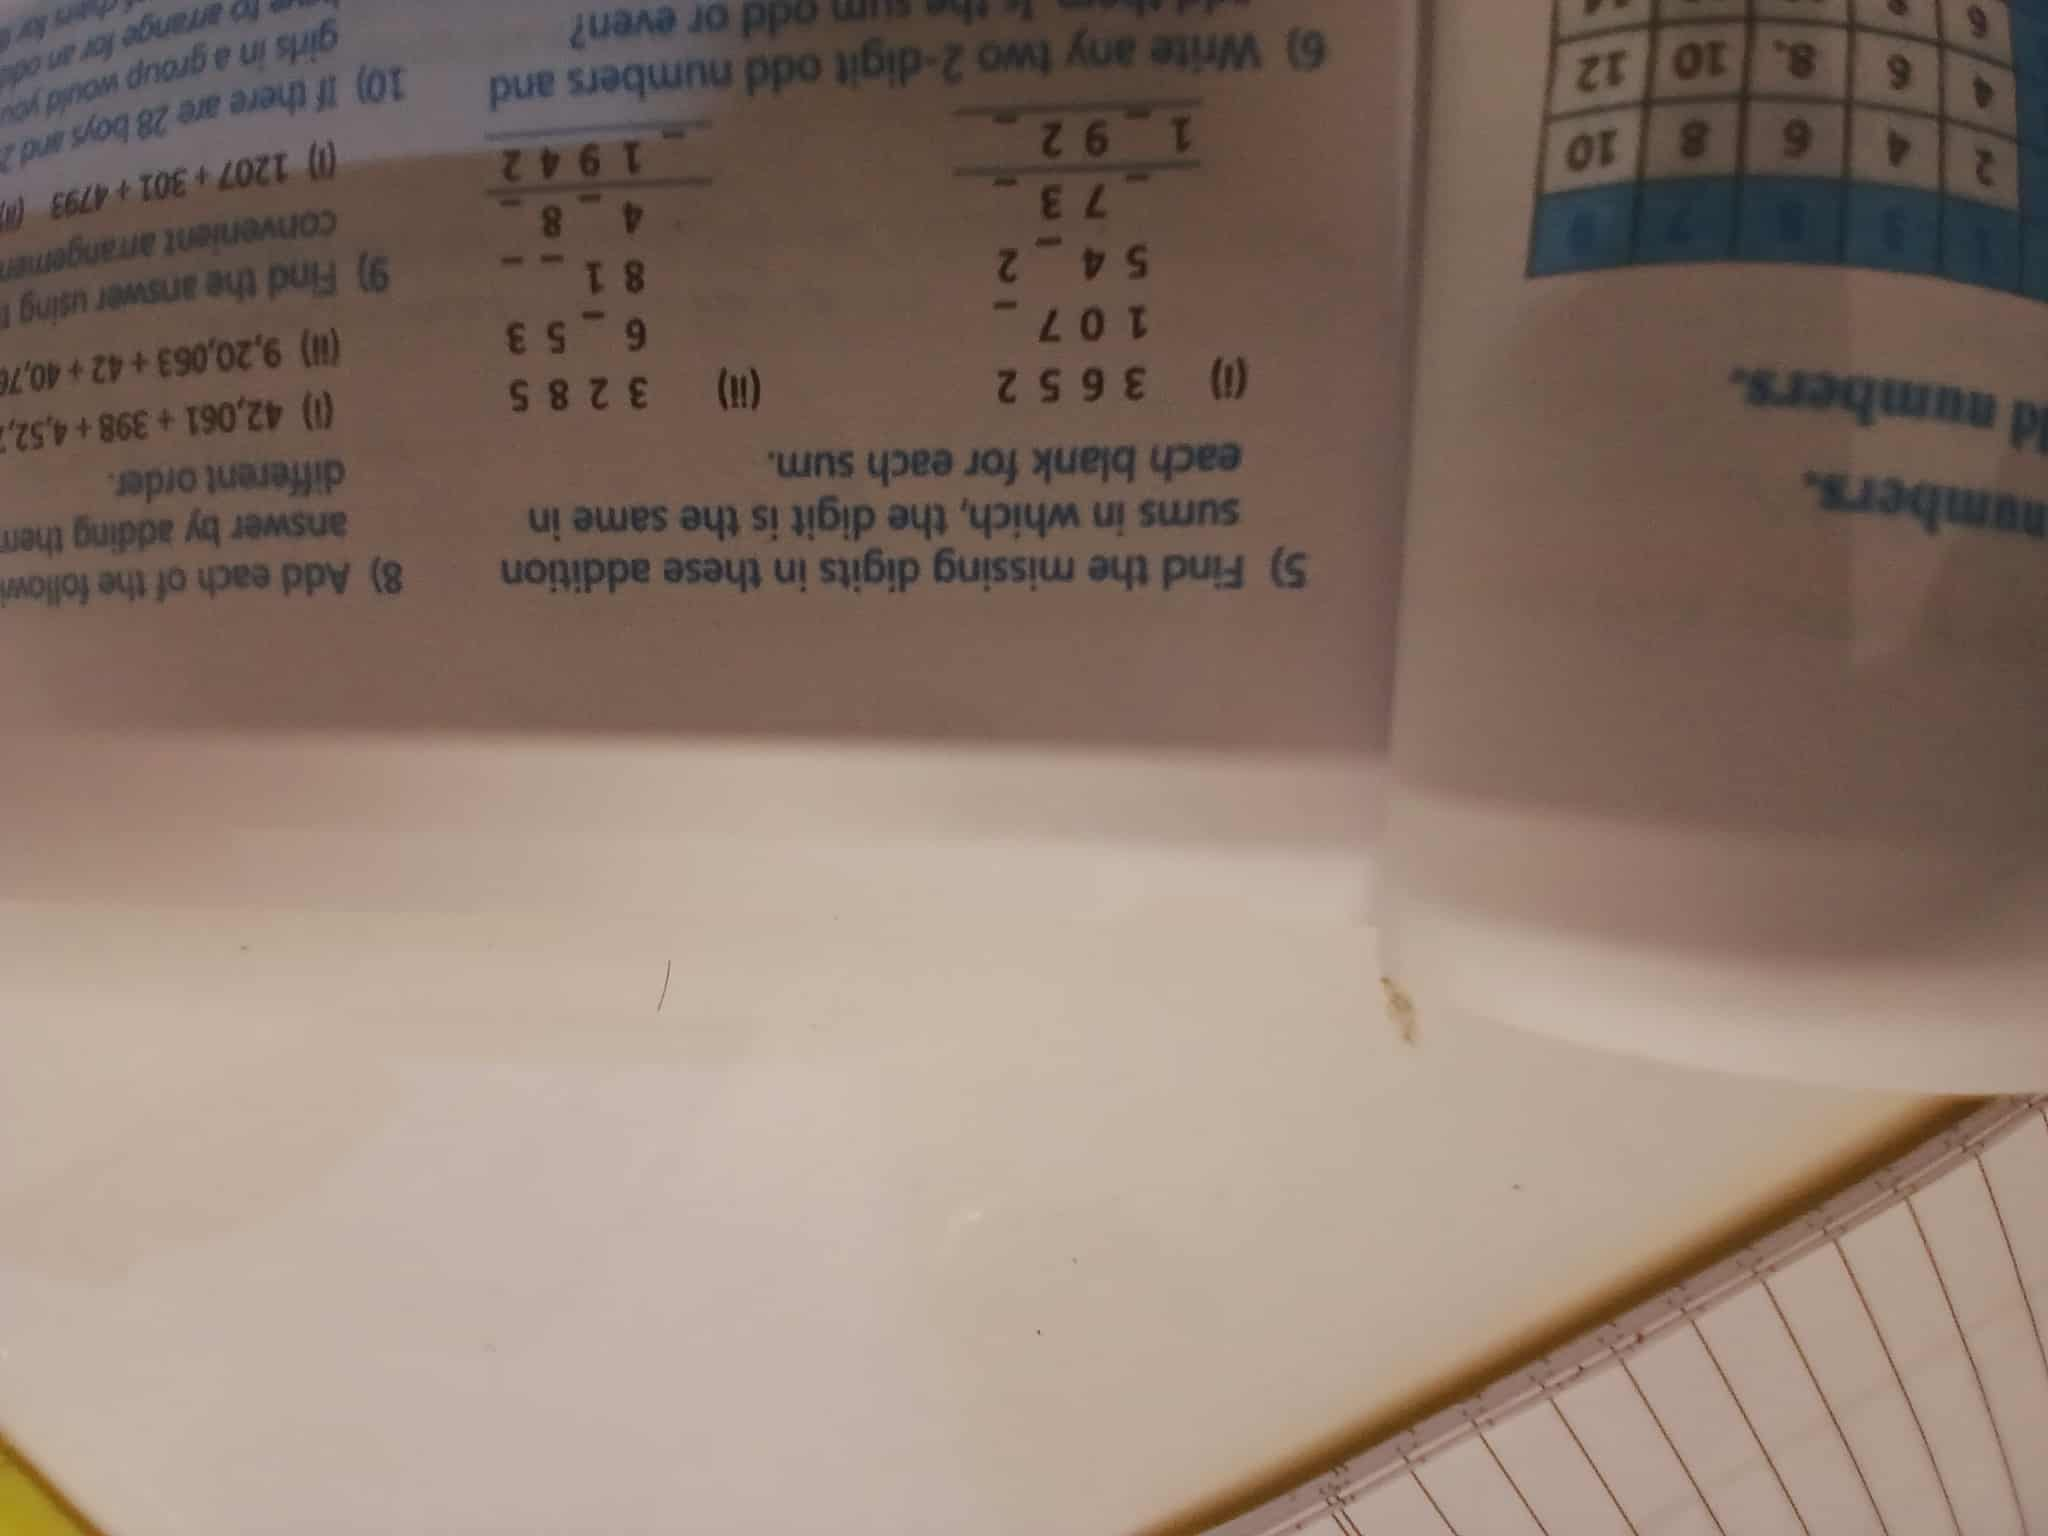
\includegraphics[width=\textwidth]{outputA.png}
    \caption{Output A}
    \label{fig:outputA}
  \end{subfigure}
  \hfill % Adds horizontal stretching space between the figures
  \begin{subfigure}{0.3\textwidth}
    \centering
    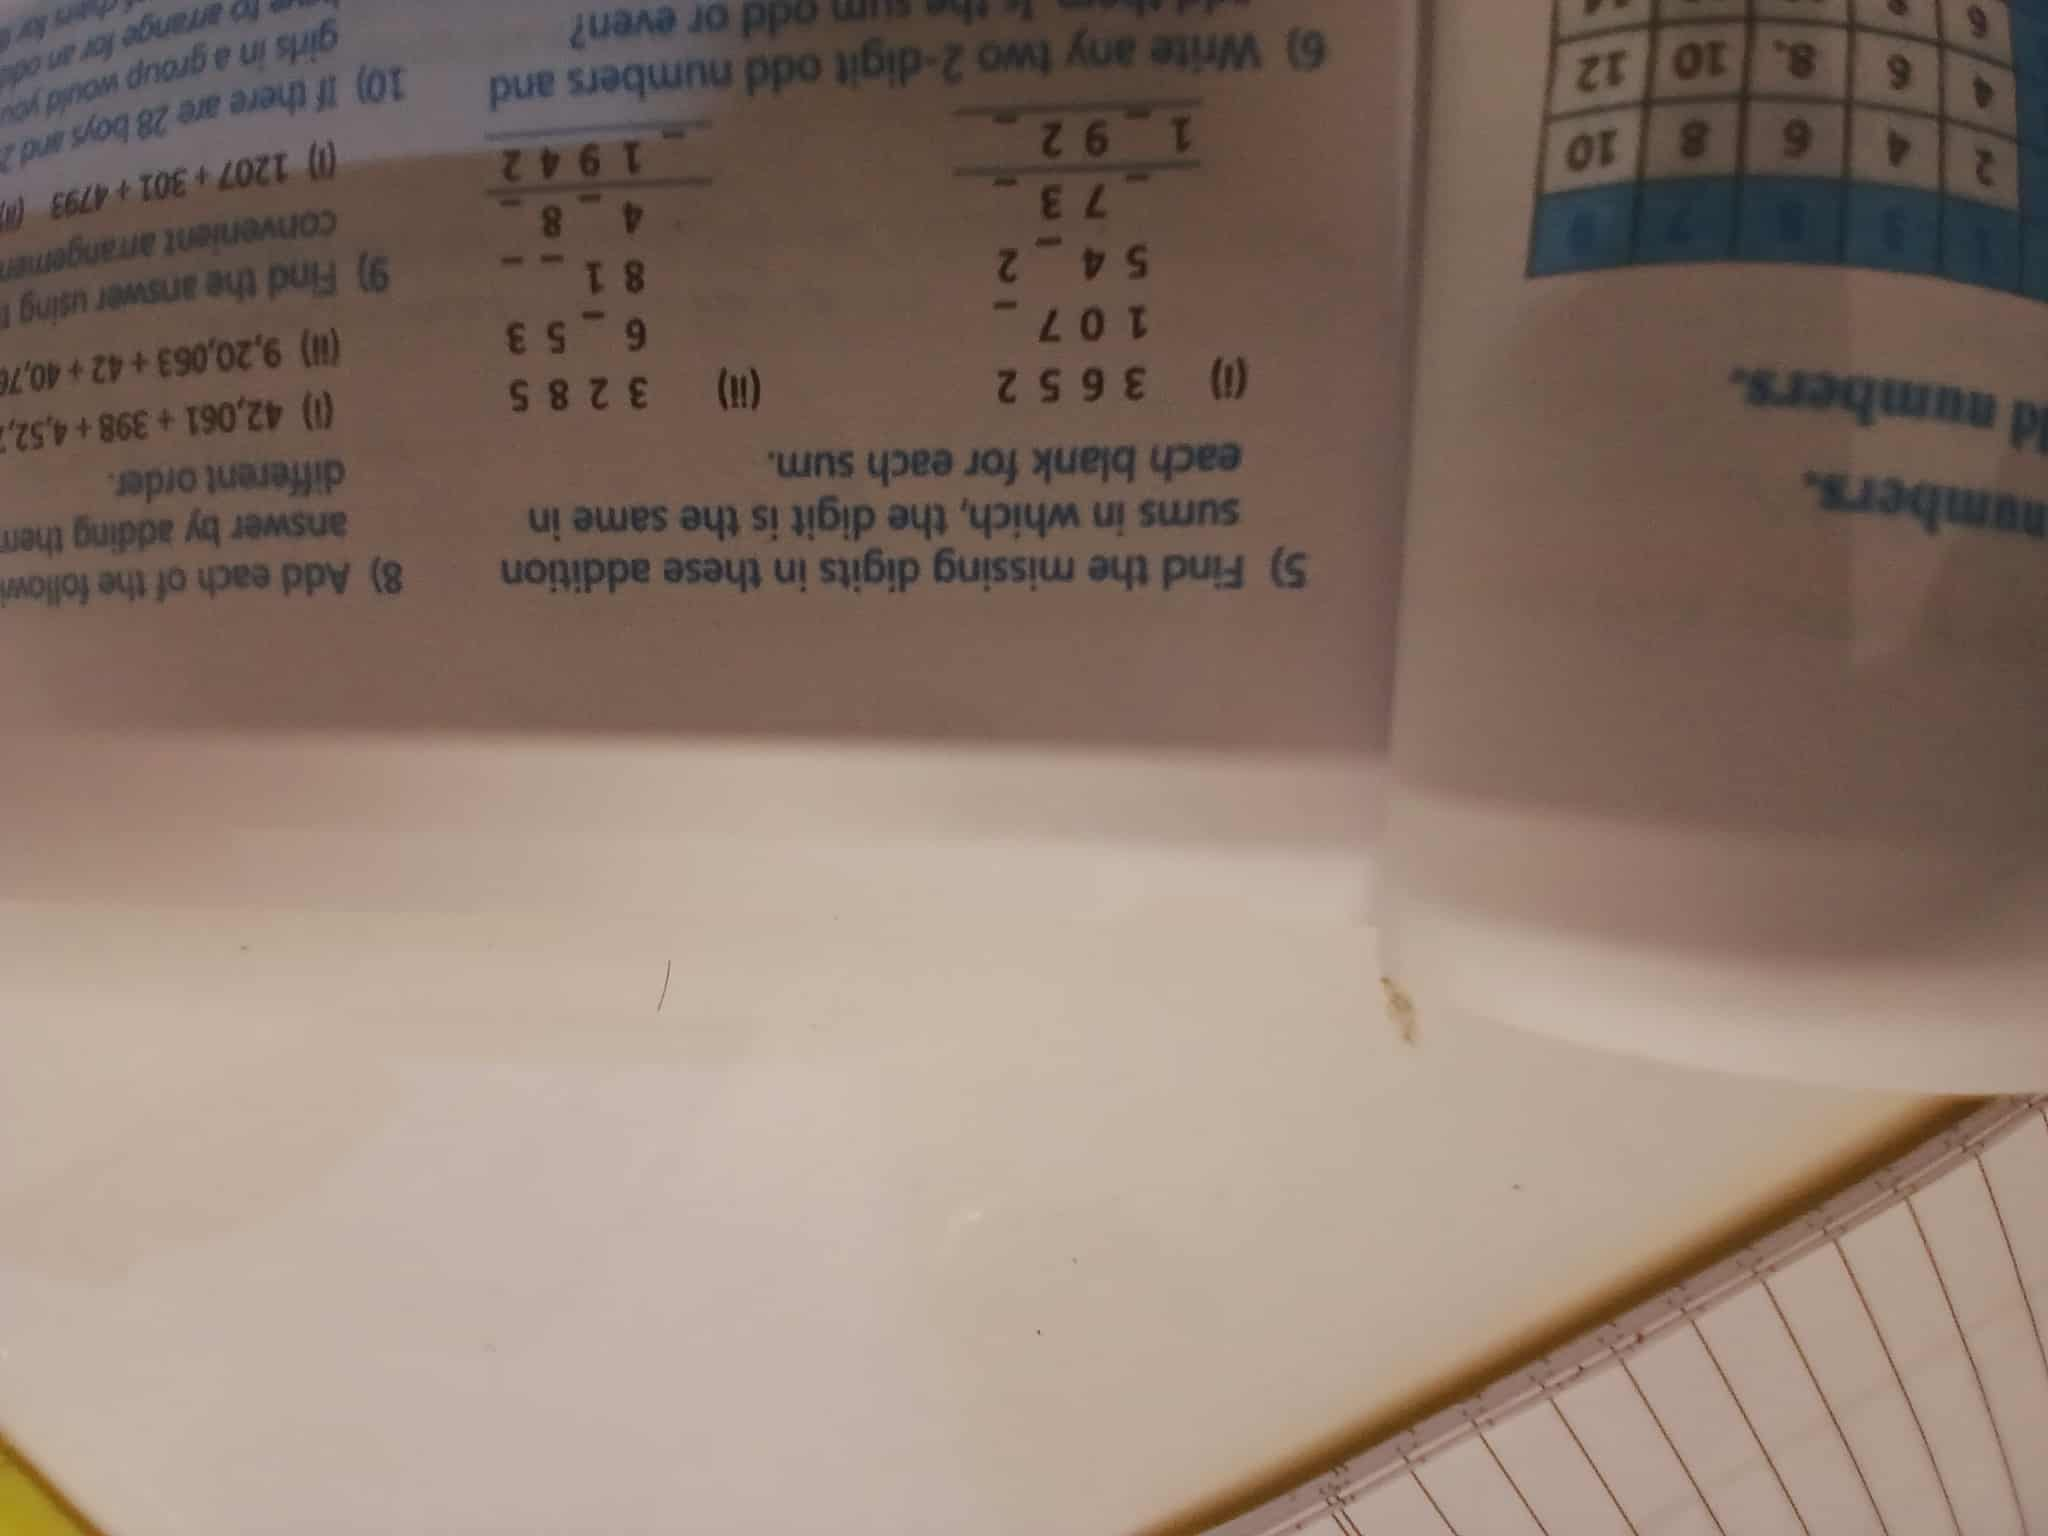
\includegraphics[width=\textwidth]{outputB.png}
    \caption{Output B}
    \label{fig:outputB}
  \end{subfigure}
  \hfill
  \begin{subfigure}{0.3\textwidth}
    \centering
    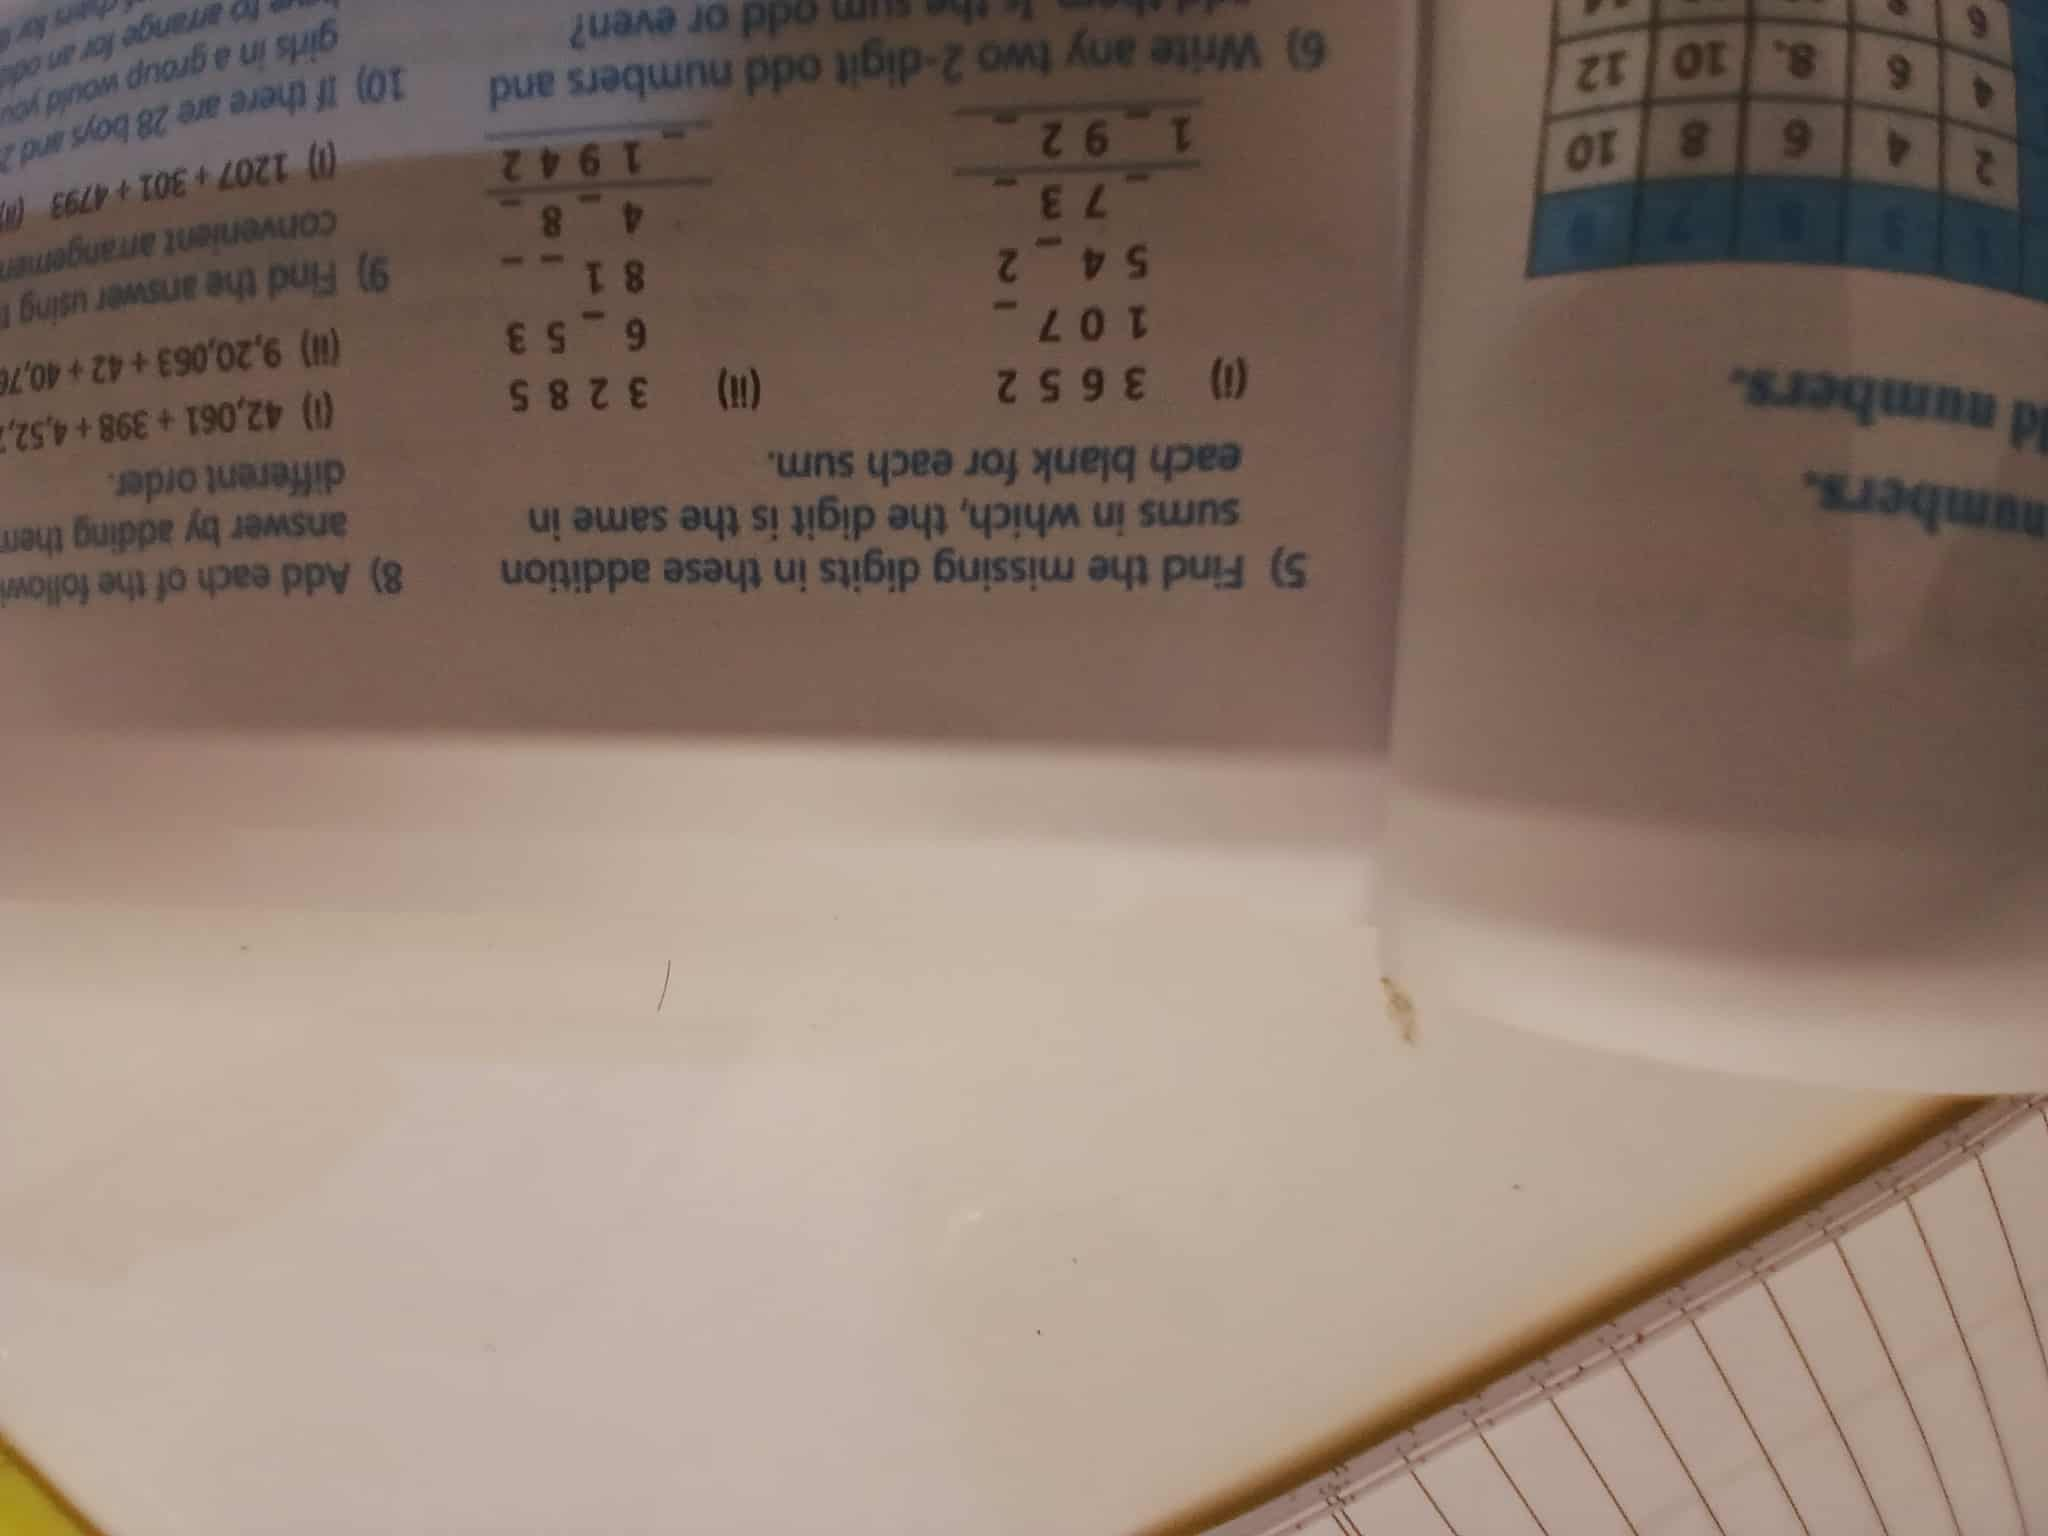
\includegraphics[width=\textwidth]{outputC.png}
    \caption{Output C}
    \label{fig:outputC}
  \end{subfigure}
  \caption{Comparison of three rendering outputs.}
  \label{fig:comparison}
\end{figure}



\begin{figure}[h]
  \centering
  \begin{subfigure}{0.5\textwidth}
    \centering
    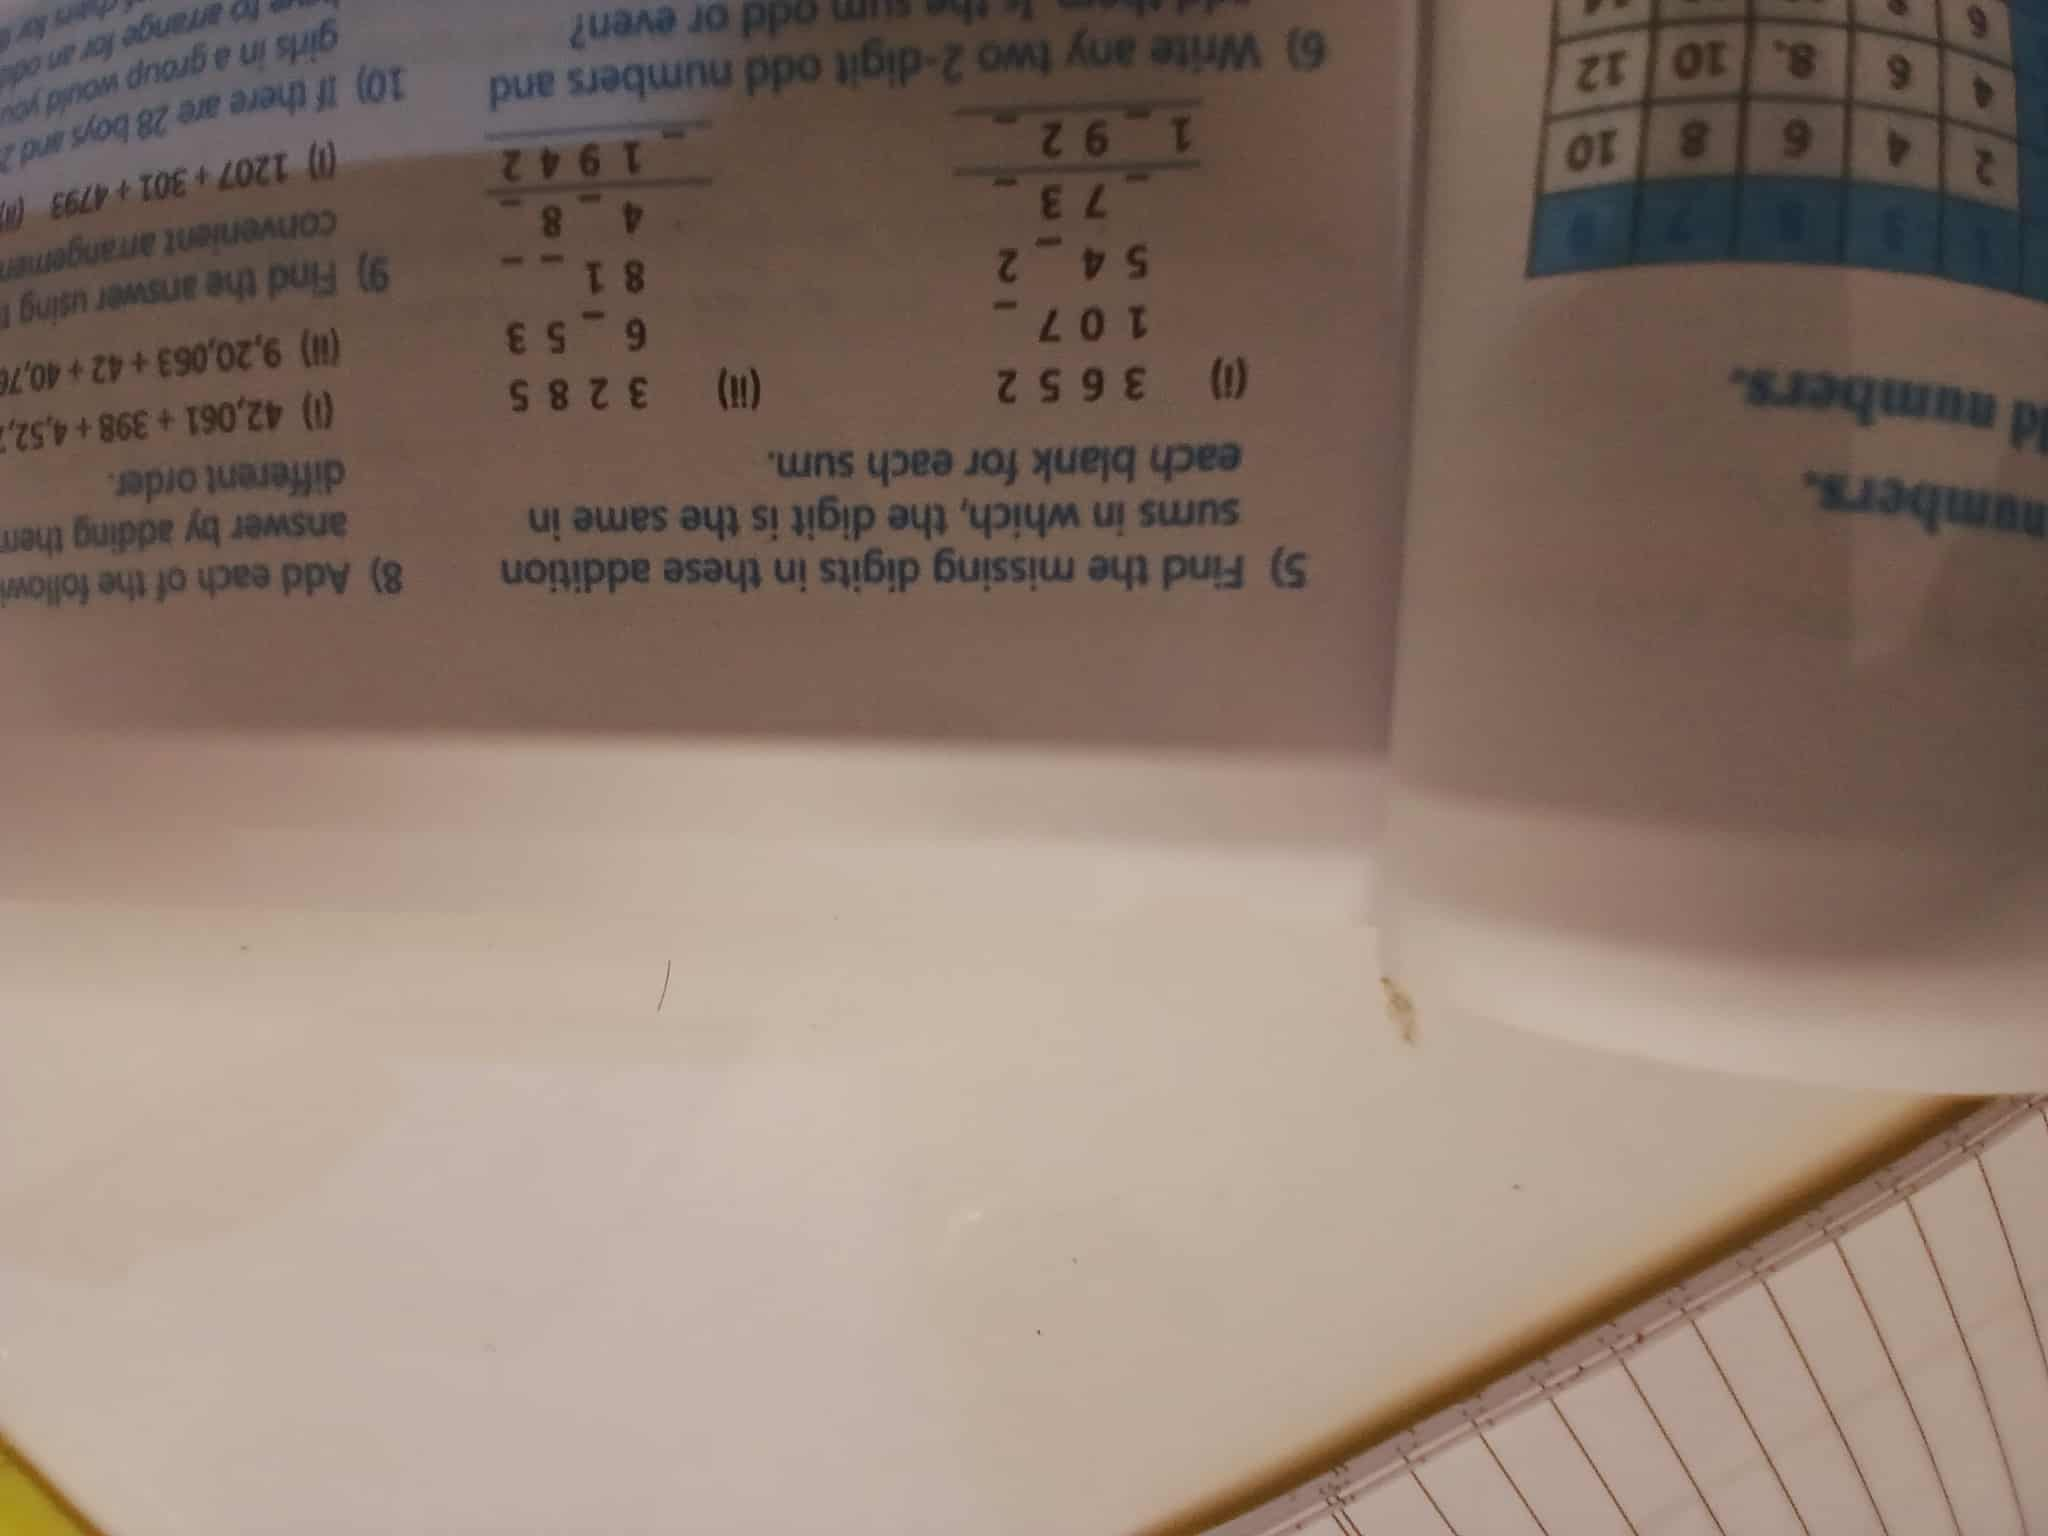
\includegraphics[width=\textwidth]{outputA.png}
    \caption{Main Diagram}
    \label{fig:main}
  \end{subfigure}

  \vspace{0.5cm}

  \begin{subfigure}{0.4\textwidth}
    \centering
    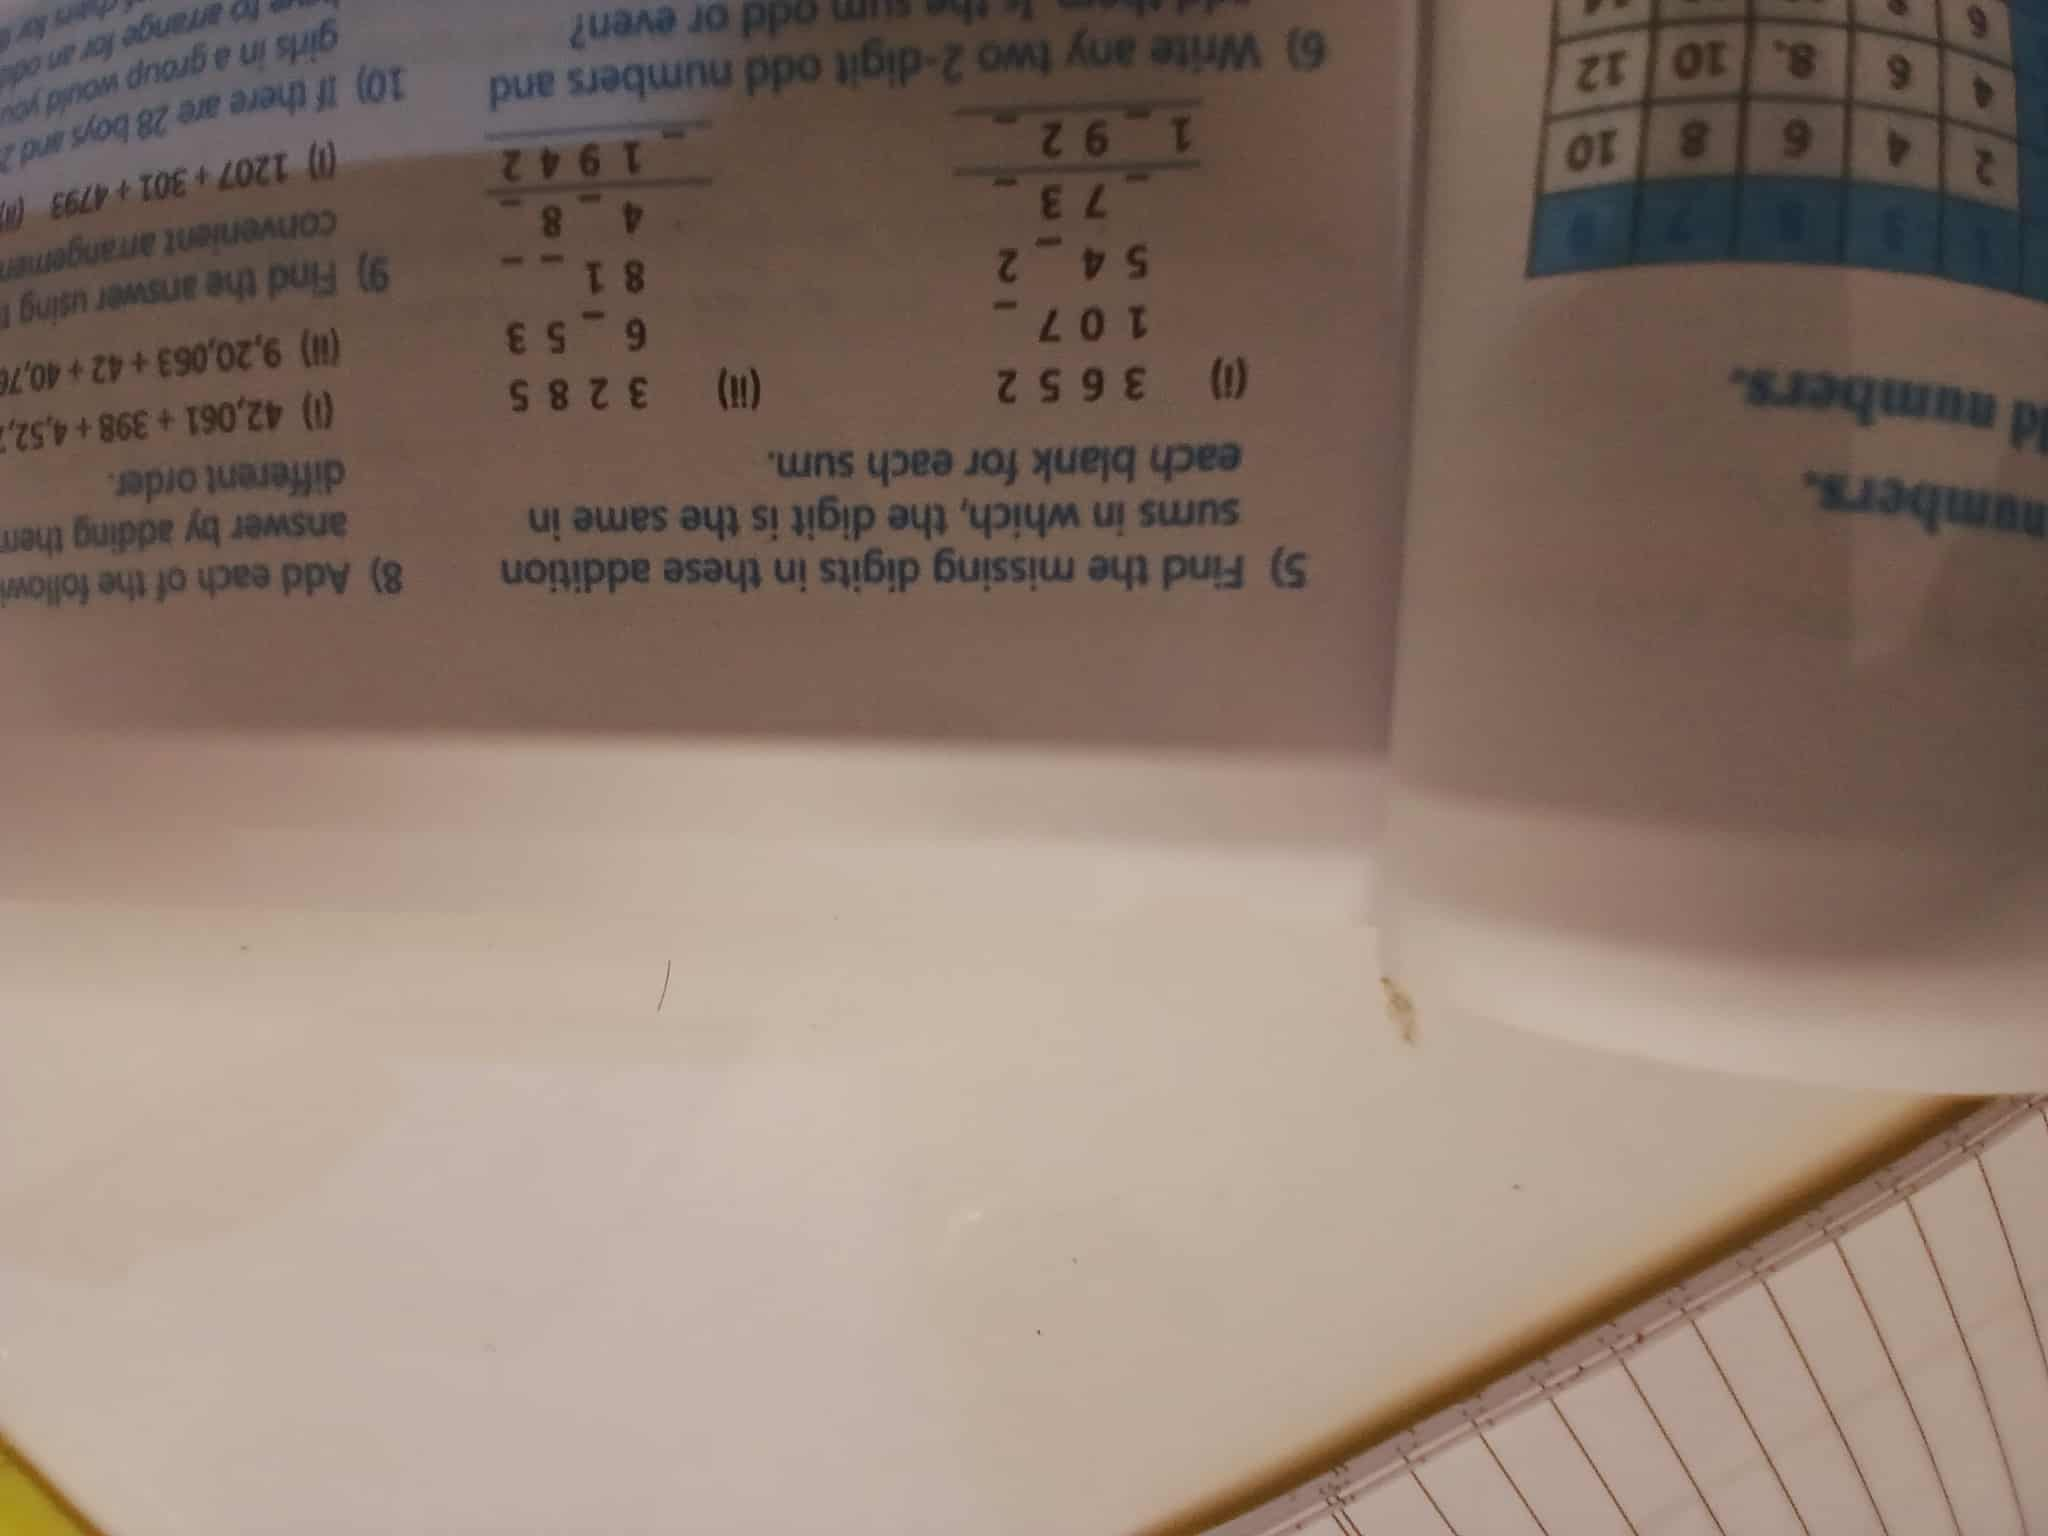
\includegraphics[width=\textwidth]{outputB.png}
    \caption{Detail B}
    \label{fig:detailB}
  \end{subfigure}
  \hfill
  \begin{subfigure}{0.4\textwidth}
    \centering
    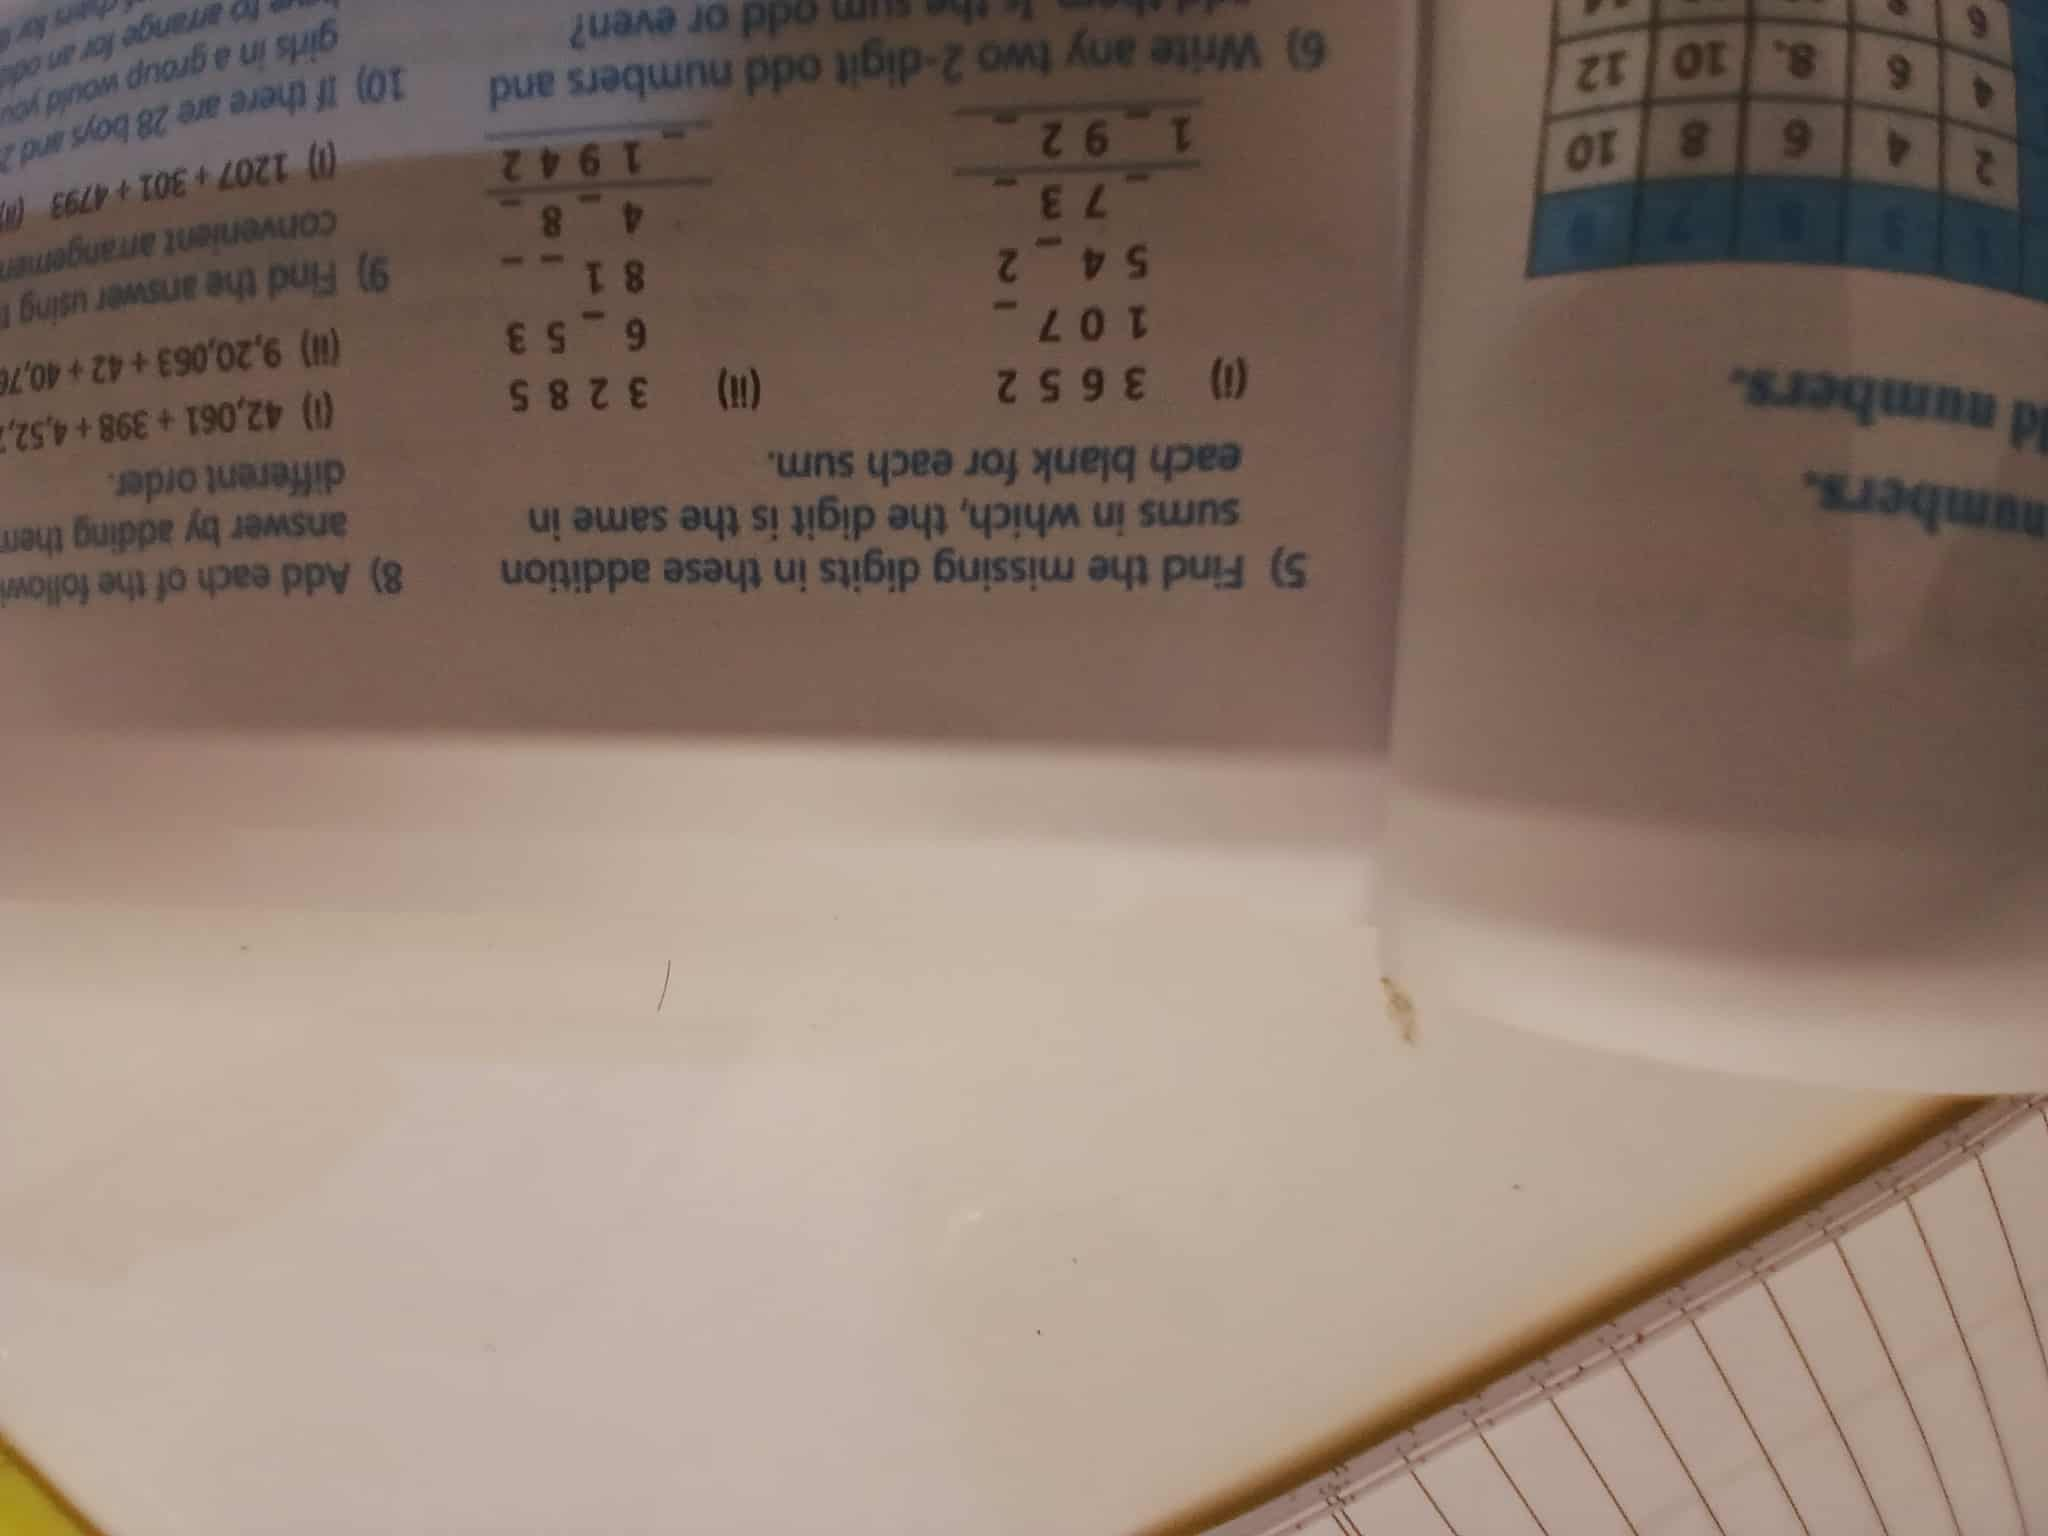
\includegraphics[width=\textwidth]{outputC.png}
    \caption{Detail C}
    \label{fig:detailC}
  \end{subfigure}
  \caption{Asymmetric layout with one dominant figure}
  \label{fig:asymmetric}
\end{figure}

\end{document}